\documentclass[oneside,final,14pt]{extreport}

% Изменяем шрифт
\usepackage{fontspec}
\setmainfont{Times New Roman}
\listfiles

% Полуторный интервал
\linespread{1.6}

% Математика
\usepackage{mathtools}

% Картинки
\usepackage{graphicx}
\usepackage{subcaption}

% Языковой пакет
\usepackage[russianb]{babel}

% Меняем класс enumerate,
% чтобы использовать кирилицу
% как маркеры
\usepackage{enumitem}
\makeatletter
\AddEnumerateCounter{\asbuk}{\russian@alph}{щ}
\makeatother

% Работа с отступами
\usepackage{vmargin}
\setpapersize{A4}
% отступы
%\setmarginsrb 
%{3cm} % левый
%{2cm} % верхний
%{1cm} % Правый
%{2cm} % Нижний
%{0pt}{0mm} % Высота - отступ верхнего колонтитула
%{0pt}{0mm} % Высота - отступ нижнего  колонтитула

% Красная строка в начале главы
\usepackage{indentfirst}

% Убиваем перенос
\usepackage[none]{hyphenat}

% выравнивание по ширине
\usepackage{microtype}

% Границы
\setlength\hoffset{0cm}
\setlength\voffset{0cm}
\usepackage[top=2cm, bottom=2cm, left=3cm, right=2cm,
]{geometry}
 		
% Настройка  заглавий
\usepackage{titlesec}

%\titleformat
%{\chapter} % command
%[display]
%{
%\bfseries
%} % format
%{
%\thechapter.
%} 	% label
%{ 
%	0 pt
%} % sep
%{    
%\centering
%} % before-code

\titleformat{\chapter}
            {\bfseries}
            {\thechapter.\hspace{1em}}
            {0pt}
            {\centering
            \vspace{0mm} }
            [\vspace{14pt}]% Отступ после
\titlespacing{\chapter}{0pt}{-50pt}{0pt}

%\titleformat{\section}
%            {\bfseries}
%            {\thechapter.\hspace{1em}}
%            {0pt}
%            {\centering
%            \vspace{0mm} }
%            [\vspace{14pt}]% Отступ после
%\titlespacing{\section}{0pt}{-50pt}{0pt}

% Конец настройка заглавий


% веелечина отступа
%\setlength\parindent{4pt}

% Добавить точки в оглавление
\usepackage{tocstyle}
\newcommand{\autodot}{.}


\sloppy
\usepackage{layout}
%% my command
\newcommand{\picPath}{pictures}
\begin{document}

\tableofcontents
\newpage
\chapter*{Введение}
\addcontentsline{toc}{chapter}{Введение}

	В Сибирском государственном университете телекоммуникаций и информатики,с которым у КубГУ имеется соглашение о сотрудничестве в сфере образования, науки, научной и инновационной деятельности стоит задача оценивания
качества контактной работы, реализуемой посредством вебинаров, в ходе дистанционного обучения. 

Для решения этой задачи разработана математическая модель, которая включает систему из 32 показателей качества организации и проведения вебинара (перечень которых представлен в приложении), позволяющих оценить с разных сторон  качество вебинара 10-балльными экспертными оценками. Проблема заключается в существенных трудозатратах, которые несут эксперты при оценивании этих показателей. Кроме того, мнения экспертов субъективны, а задача поставлена максимально объективизировать процедуру оценивания, например, за счет минимизации влияния человеческого фактора в процедуре оценивания. В связи с этим актуальной является  задача разработки такой компьютерной технологии, которая позволит оценить максимальное количество показателей без участия человека в автоматическом режиме. В числе показателей, которые могут быть автоматически при помощи некоторого алгоритма входят: колличество и качество информации на слайдах, использование указки, точность заявленной длительности мероприяти и тд.

Основой для анализа данных показателей является три основных аспекта:
%\begin{enumerate}[label=\asbuk*),ref=\asbuk*, noitemsep]
\begin{itemize}[label= $-$, noitemsep]
\item поиск указки
\item выделение слайдов
\item Распознавание блоков текста на слайдах
\end{itemize}
%\end{enumerate}
 
Для решения данных задач в ходе курсовой работы были рассмотрены алгоритмы поиска границ обектов на изображении, сравнения двух изображений, поиска шаблона в изображении, а также методы локализации текста среди прочих объектов. Кроме того, изучены методы, которые позволяют значительно ускорить работу всех вышеперечисленных алгоритмов. Програмно было реализованны процедуры, реализующие основу для дальнейшего развития приложения автоматического вычисления некоторых показателей вебинаров. 

\chapter{Методы определения границ объектов на изображении}
Границы объектов на изображении характеризуются изменением яркости в некотором направлении. Выделяют три вида границ: идеальные,  размытые  и крышевидные. На рис № изображены вертикальные границы трех видов.

\begin{figure}[h!]
  \centering
  \begin{subfigure}[b]{0.4\linewidth}
    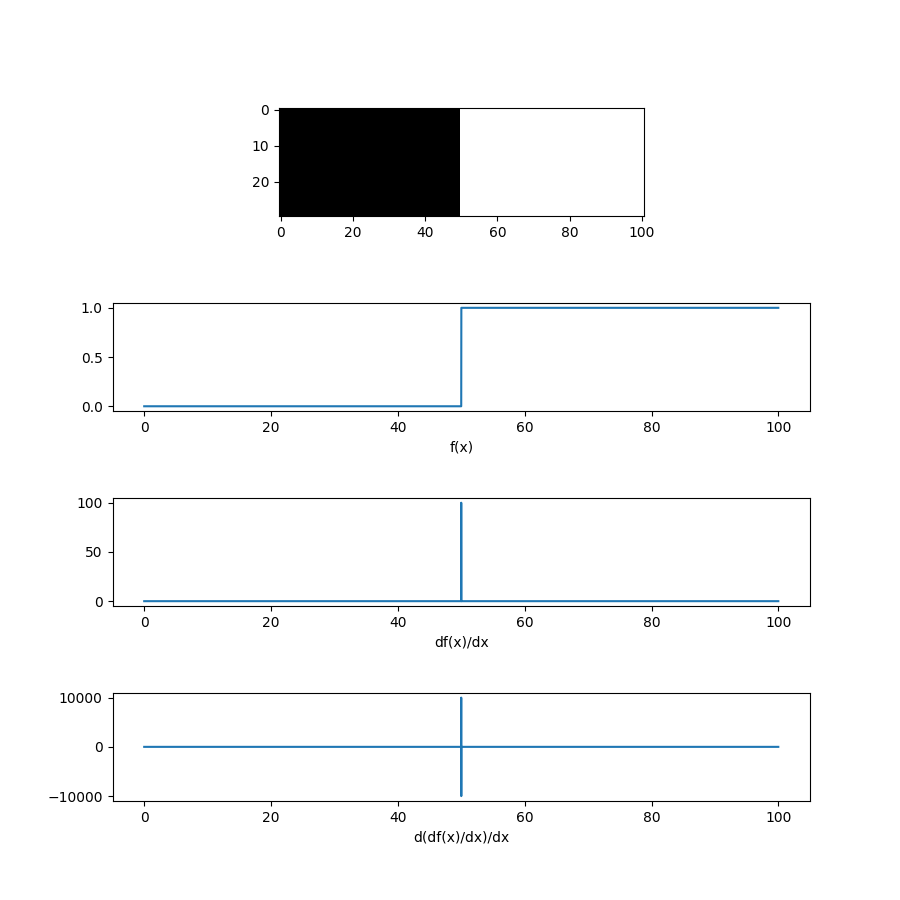
\includegraphics[width=\linewidth]{\picPath/perfect.png}
    \caption{ идеальная граница}
  \end{subfigure}
  \begin{subfigure}[b]{0.4\linewidth}
    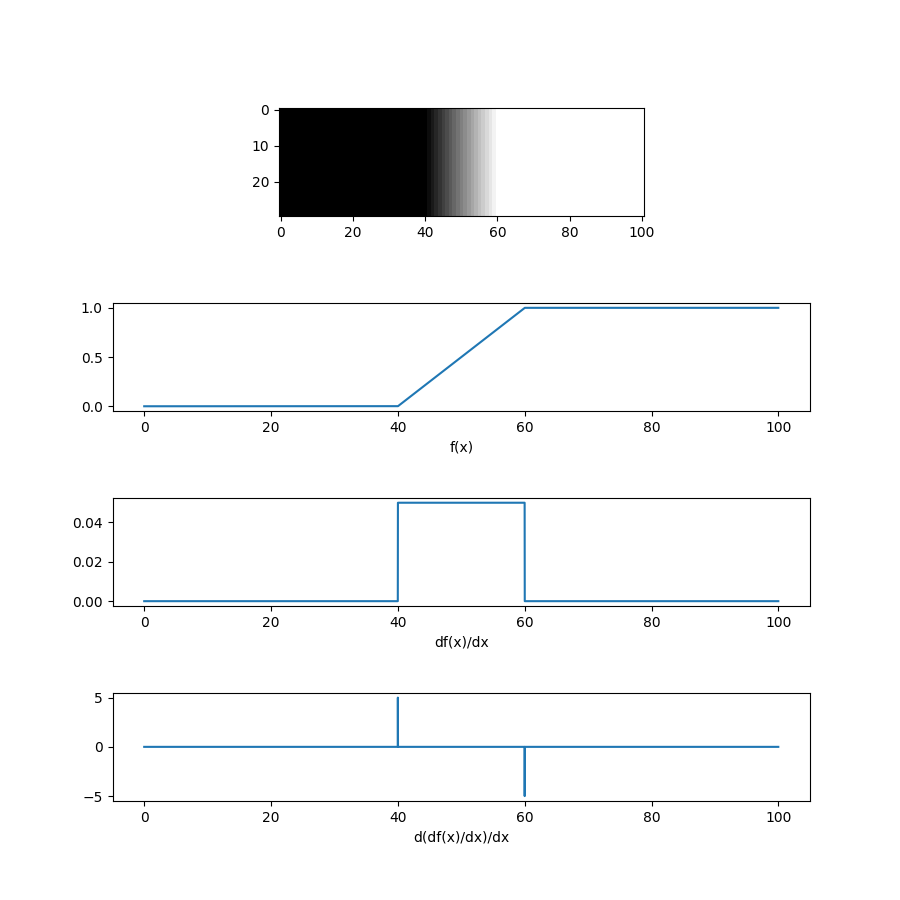
\includegraphics[width=\linewidth]{\picPath/smooth.png}
    \caption{размытая граница}
  \end{subfigure}
  \begin{subfigure}[b]{0.4\linewidth}
    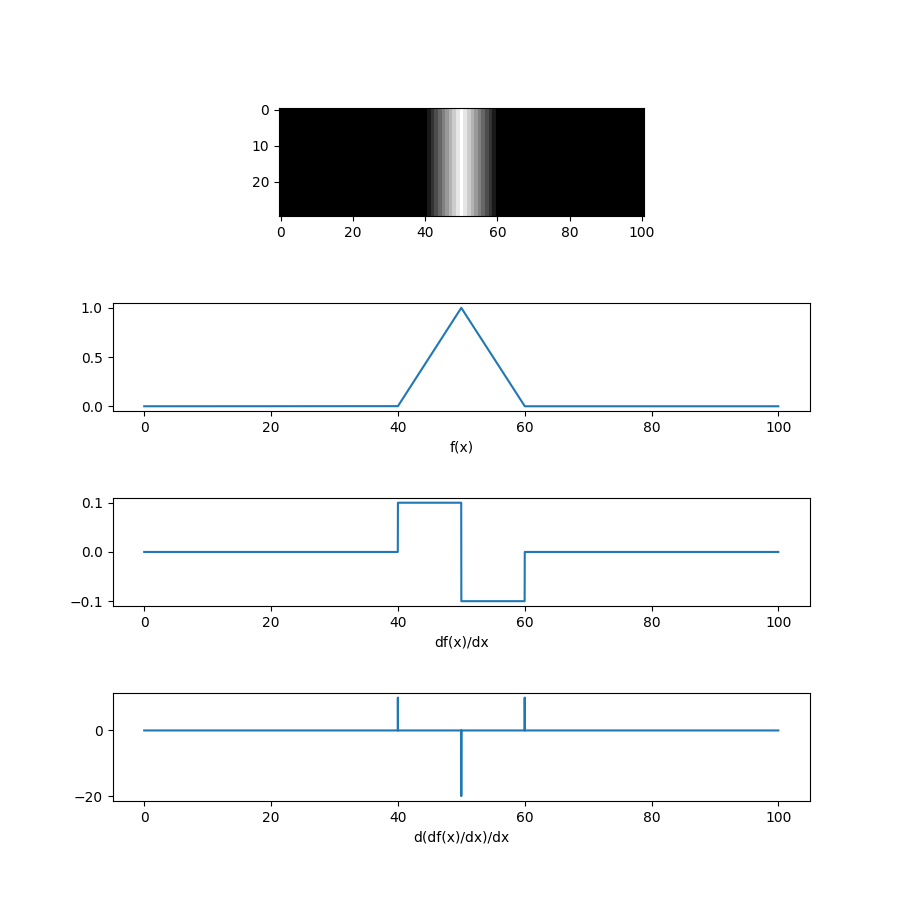
\includegraphics[width=\linewidth]{\picPath/roof.png}
    \caption{крышевидная граница}
  \end{subfigure}
  \caption{The same cup of coffee. Two times.}
  \label{fig:coffee}
\end{figure}

Рассмотрим вертикальную размытую границу. Тогда зафиксировав ординату, получим дискретную функцию от одной переменной $g(x)$. Рассмотрим её первую и вторую производные: первая производная равна нулю в областях, где интенсивность постоянна и равна константе на границе, причем константа тем больше, чем уже граница. Вторая производная не равна нулю только в координатах начала и конца границы $g(x)$ В этих точках она равна бесконечности. Для случая крыловидной границы, первая производная положительна на подъеме и отрицательна на спуске границы. Вторая производная не ноль в трех точках, причем граница помещается между первой и последней не нулевой точкой второй производной. Отсюда следует вывод: зная направление границы, её координаты находятся из производной функции интенсивности по этому направлению. 
 
В общем случае, если заранее неизвестны направления границ объектов, за направление берут направление максимального роста интенсивности  т.е. градиент изображения, если представлять его как дискретную функцию от двух переменных. 

Градиент есть вектор частных производных.
\begin{equation}
\nabla f(x,y) 
= 
grad[f(x,y)]
=
\begin{bmatrix}
g_x(x,y)\\
g_y(x,y)
\end{bmatrix}
=
\begin{bmatrix}
\frac{\partial f(x,y)}
{\partial x}\\
\frac{\partial f(x,y)}
{\partial y}
\end{bmatrix}
\end{equation}

 На практике производные вычисляются численно, разностными методами. Если принять расстояние между соседними в строке и соседними в столбце пикселями за единицу, компоненты градиента с точностью $O(1)$ вычисляется по формулам

\begin{gather}
g_x(x,y) 
= 
\frac{\partial f(x,y)}
{\partial x}
=
f(x+1,y) - f(x,y)
\\
g_y(x,y) 
= 
\frac{\partial f(x,y)}
{\partial y}
=
f(x,y+1) - f(x,y)
\end{gather}
Что равносильно свертке изображения с ядрами 
\begin{equation}
\begin{bmatrix}
-1\\1
\end{bmatrix}
\quad
\begin{bmatrix}
-1 & 1
\end{bmatrix}
\end{equation}
На практике для вычисления градиента используются оператор Собеля
\begin{equation}
\begin{bmatrix}
 -1 & \,2 & -1 \\
\,0 & \,0 &\,0 \\
\,1 & \,2 &\,1
\end{bmatrix}
\quad
\begin{bmatrix}
-1 & 0 &  1 \\
-2 & 0 &  2 \\
-1 & 0 &  1
\end{bmatrix}	
\end{equation}
Конечное изображене вычисляется 	по формуле
\begin{equation}
G
=
|G_x| + |G_y|
\end{equation}
В результате получаем чб изображение, на котором белым цветом изображены предполагаемые границы.

\chapter{Методы сравнения изображений}
\section{Сравнение гистограмм}
Один из самых простых и быстрых способов сравнения  двух изображений. Основан на предположении о том, что похожие изображения имеют похожие цвета. 

Гистограмма - график  или функция распределения элементов цифрового изображения с различной яркостью. Определена на множестве всех возможных значений яркостей ч.б. изображения, значение функции равно количеству пикселей, яркость которых равна аргументу гистограммы. В общем случае значение яркости может быть вектором. Обычно для сравнения цветных изображений используются каналы HS цветового пространства HSV. Объясняется это тем, что при сравнении цвета разной яркости не различают, а поэтому канал V, отвечающий за яркость цвета игнорируют.  

Для сравнения гистограмм в openCV используется одна из метрик

Correlation  CV\_COMP\_CORREL
 
$$
d(H_1,H_2) 
= 
\frac{
\sum_I(H_1(I) - \overline{H}_1)
(H_2(I)-\overline{H}_2)
}{
	\sqrt{
		\sum_I(H_1(I) - \overline{H}_1)^2
		\sum_I(H_2(I) - \overline{H}_2)^2
	}
}
$$
$$
\overline{H}_k 
= 
\frac{1}{N}
\sum_J H_k(J)
$$

Chi-Square ( CV\_COMP\_CHISQR )
$$
d(H_1,H_2)
=
\sum_I \frac{
	(H_1(I) - H_2(I))^2}
{H_1(I)}
$$

Intersection ( method=CV\_COMP\_INTERSECT )

$$
d(H_1,H_2)
=
\sum_I 
\min (H_1(I),H_2(I))
$$

Bhattacharyya distance ( CV\_COMP\_BHATTACHARYYA )
$$
d(H_1,H_2)
=
\sqrt{ 1 - 
\frac{1}{
  \sqrt{\overline{H}_1 
  		\overline{H}_2
  		N^2}
  }
  \sum_I
  \sqrt{H_1(I) H_2(I)}
}
$$

$I$ в общем случае вектор, сумма идет по всем возможным векторам.


Тут таблица с результатами

Плюс данного метода - инвариантность относительно формы и размера сравниваемых изображений.

Главный недостаток метода сравнения гистограмм -   разделение изображений весьма условно. Каждому изображению подобно всё множество изображений, составленных из тех же пикселей, расположенных в произвольном порядке. Поэтому данный метод не подходит, например,  для задачи поиска курсора т.к. существует вероятность того, что на изображении, кроме курсора, могут находиться элементы, гистограммы которых очень близки к гистограмме курсора.   

\section{Совпадения по шаблону}
Данный класс методов используется для нахождения координат малого шаблонного изображения в большом. Алгоритм поиска таков:
На первом этапе происходит нелинейная фильтрация изображения. Как и в остальных фильтрах, для фильтрации используется скользящее окно[Ссылка на мо. предыдущую курсовую]. Размер этого окна равен размеру малого изображения. Все возможные подобласти размера окна  из большого изображения поэлементно сравниваются с малым изображением посредством одной из метрик.   

 method=CV\_TM\_SQDIFF

$$
R(x,y)
=
\sum_{x',y'}
(T(x',y')-I(x+x',y+y'))^2
$$ 

method=CV\_TM\_SQDIFF\_NORMED

$$
R(x,y)
=
\frac{
R(x,y)
=
\sum_{x',y'}
(T(x',y')-I(x+x',y+y'))^2
}
{
\sqrt{
	\sum_{x',y'}
	T(x',y')^2
	\sum_{x',y'}
	I(x+x',y+y')^2
	}
}
$$

method=CV\_TM\_CCORR

$$
R(x,y)
=
\sum_{x',y'}
( T(x',y')I(x+x',y+y'))
$$

method=CV\_TM\_CCORR\_NORMED

$$
R(x,y)
=
\frac{
	\sum_{x',y'}
	( T(x',y')I(x+x',y+y'))
}
{
	\sum_{x',y'}
	T(x',y')^2
	\sum_{x',y'}
	I(x+x',y+y')^2
}
$$

На втором этапе полученная двумерная матрица нормируется. и в зависимости от используемого метода находится её минимальный или максимальный элемент.

\begin{figure}[h!]
  \centering
  \begin{subfigure}[b]{0.09\linewidth}
    
\includegraphics[width=\linewidth]{\picPath/cursor.png}
    \caption{ идеальная граница}
  \end{subfigure}
  \begin{subfigure}[b]{0.4\linewidth}
    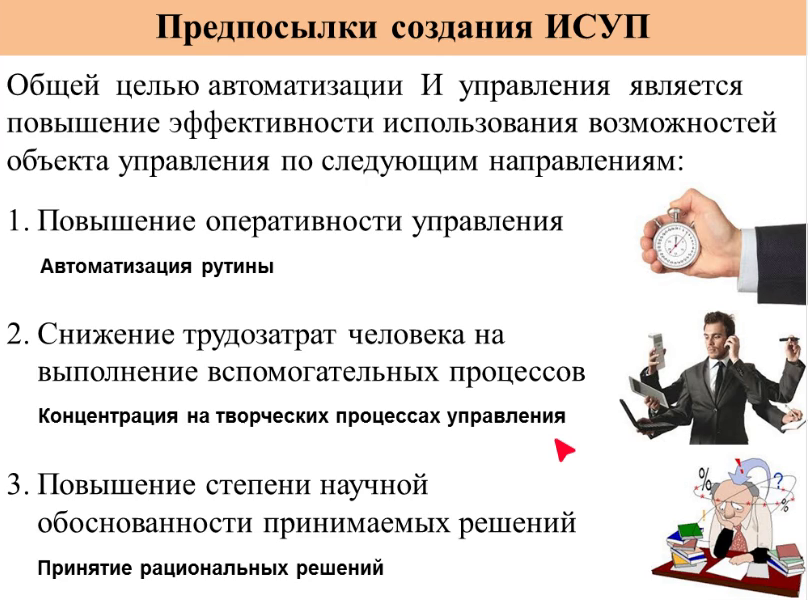
\includegraphics[width=\linewidth]{\picPath/tmpl_matching_inp.png}
    \caption{размытая граница}
  \end{subfigure}
  \begin{subfigure}[b]{0.4\linewidth}
    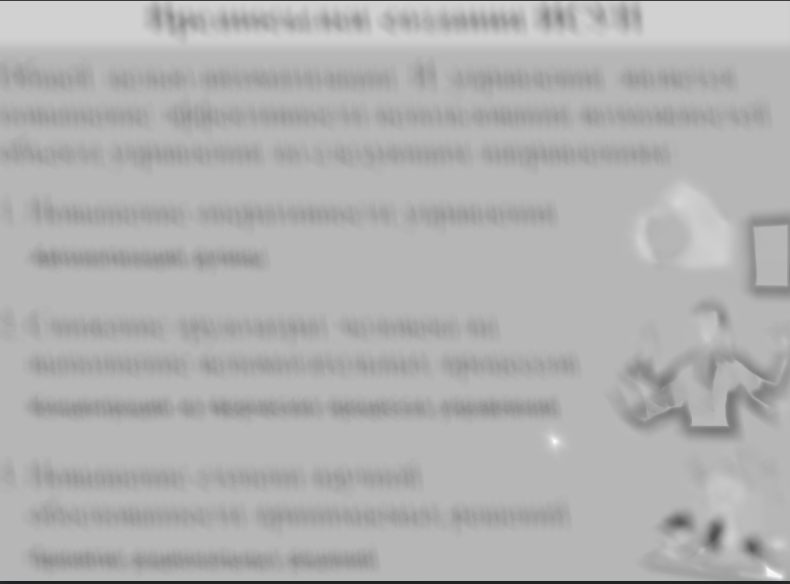
\includegraphics[width=\linewidth]{\picPath/match_template_mask.png}
    \caption{крышевидная граница}
  \end{subfigure}
  \begin{subfigure}[b]{0.4\linewidth}
    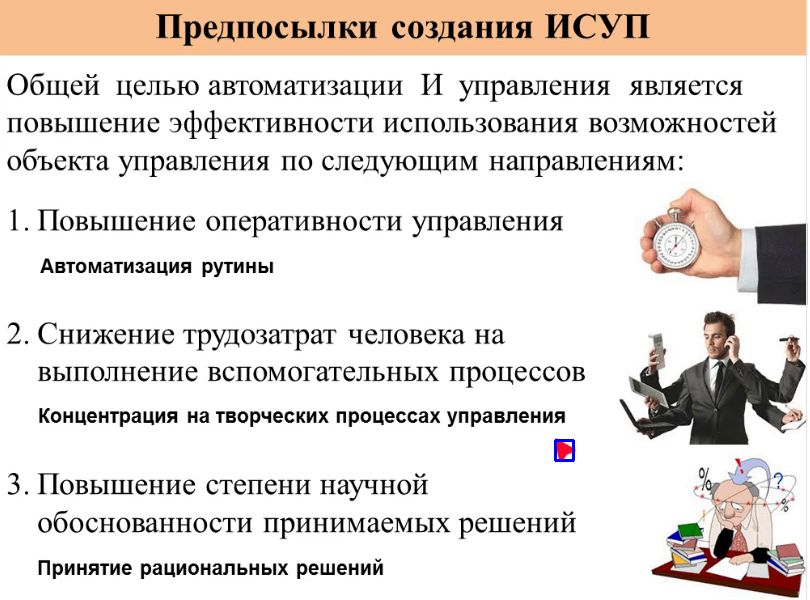
\includegraphics[width=\linewidth]{\picPath/templ_matching_result.png}
    \caption{крышевидная граница}
  \end{subfigure}
  \caption{The same cup of coffee. Two times.}
  \label{fig:coffee}
\end{figure}

Достоинства метода  - высокая точность нахождения фрагментов изображений.

Недостатки - высокая точность достигается только в случае, когда фрагмент того же размера и не повернут относительно шаблона. 
	
	Методы, инвариантные относительно размера и положения искомого элемента и перспективы называются методами совпадения по признакам. Суть методов заключается в том, что из шаблонного изображения выделяются некоторые характерные признаки. После, в большом изображении находится объекты, схожие по признакам с шаблоном.
	
\chapter{Дискретное преобразование Фурье}
Для анализа аналоговых и цифровых сигналов зачастую используются дискретные преобразования, переводящие сигнал из одного базиса в другой. Многие операции над сигналом значительно упрощаются в частотном базисе, позволяя ускорить алгоритмы машинного зрения. Рассмотренные ниже преобразования представляют сигнал в виде суперпозиции частот. 
[4]
Непрерывное преобразование Фурье имеет вид:

\chapter{ Приложения преобразования Фурье }
\section{Свертка изображений}

Как было показано выше, свертка двух функций в пространственном базисе эквивалентна по элементному произведению в частотном. В Частности, в случае изображений: вместо очевидного метода свертки, когда окно скользит по изображению и на каждой итерации вычисляется значение пикселя, можно перевести изображение и ядро фильтра в частотный базис посредством прямого преобразования Фурье, выполнить скалярное произведение двух образов и последним шагом преобразовать произведения образов в пространственный базис с помощью обратного преобразования Фурье. 

Очевидный метод требует MNmn операций для свертки изображения размера MxN с ядром размерности mxn. Свертка же посредством преобразования Фурье, вместе со всеми преобразованиями требует 2MNlog2(MN) Операций, что в случае большой размерности ядра значительно уменьшает число вычислений. 

Пример - Гаусовский фильтр:
Картинка девушки, картинка фильтра в пиксельном базисе
Картинка девушки, картинка фильтра в частотном базисе
Результат произведения, результат обратного преобразования.

\section{Алгоритм быстрой  кросс кореляции [5]}
Данный алгоритм  - разновидность поиска по шаблону. Главное его отличие в том, что для метрика представляет из себя корелляцию. Из теоремы о корелляции известно, что ...  

Что значит, что для нахождения шаблона в изображении можно использовать преобразование Фурье и значительно уменьшить количество вычислений. 
Рассмотрим метрику вида.

\begin{equation}
\gamma(u,v)
=
\frac{
\sum_{x,y}
[f(x,y) - \overline{f}_{u,v}]
[t(x-u,y-v)-t]
}
{
\sqrt{
\sum_{x,y}
[f(x,y) - \overline{f}_{u,v}]^2
\sum_{x,y}
[t(x-u,y-v)-t]^2
}
} 
\end{equation}

где
\begin{gather*}
t'(x,y)
\equiv
t(x,y) - \overline{t}
\\
f'(x,y)
\equiv
f(x,y) - \overline{f}_{u,v}
\end{gather*}

...

Тогда можем вычислить числитель как

\begin{equation}
\mathcal{F}^{-1}
\{
\mathcal{F}(f')
\mathcal{F}^*(t')
\}
\end{equation}
В знаменателе второе слагаемое всегда константа. Первое слагаемое можно вычислить, используя только 3M2   вместо 3N2(M-N+1) операций, если использовать подход бегущей суммы ( интегрирование изображений ). 
Сравнивая методы поиска шаблона можно заметить, что методы быстрой кросс корелляции рабоатет на порядок быстрее алгоритмов, не использующих преобразование Фурье. 

table

Данный алгоритм был разработан специально для фильма “Форест Гамп”(1994) и использовался в большом количестве других проектов. Во время производства фильма было необходимо вырезать и заменить некоторые части изображения из видеопотока. Шаблон вручную выделялся, а после автоматически отслеживался на протяжении всей сцены посредством ускоренной нкк. Найденные координаты использовались для дальнейших спецэффектов.

\chapter{методы локализации текста на картинке}
[6]Проблема распознавания текстовых изображений появилась давно. Системы распознавания текста из изображения (Optical Character Rectinion) нашли своё применеия во многих отраслях жизни:

\begin{itemize}[label= $-$, noitemsep]
\item Чтение регистрационных знаков транспортных средсв
\item Определение и чтение дорожных знаков

\item Мобильное приложение для слабовидящих, распознающее и проговаривающее текст из изображения

\item Ввод информации

\item Оцифровка или архивация документов, видеопотока с камеры наблюдения и тд

\end{itemize}

На сегодняшний день решена достаточно хорошо. Тем не менее, алгоритмы не могут дать 100 процентный результат т.к. входные данные могут быть подвержены искажениям. Основные из них

\begin{itemize}[label= $-$, noitemsep]
\item Низкое разрешение 


\item Неравномерное освещение

\item Георметрические искажения

\item Дисторсия

\item Сложный фон

\item Шумы итд.

\end{itemize}

Задача распознавания текста не может быть поставленна точно: в некоторых ситуациях текст не возможно распознать физически, буквы не могут быть распознанны однозначно. Этот факт не уменьшает ответсвенности, возложенной на разработчика алгоритма распознавания образов.

Первый   этап большинства алгоритмов распознавания текста - его локализация. Главное отличие текста от фона и изображенй - высокий контарст. Кроме того, текст чаще всего имеет некоторый шрифт, у которого есть постоянный размер. На изображениях  условно выделяют два вида текстовой информации: текст, который нанесен на объекты съемки т.е надписи на транспорте, вывески, реклама и текст, который нанесен поверх изображения или со скана документа и тд. 

\section{Градиентные методы локализации текста}

Исходят из предположения о том, что символы имеют четкие границы, в отличие от другой информации, а значит пиксели, значения градиента в которых велико можно интерпертировать как границы символов. Следующим этапом границы группировались в текстовые блоки.

Аналогичный подход использовали Lee и Kankanhalli, только используя вертикальную производную. Kuwano et al. объеденил предыдущие подходы: предпологал текстовые блоки по вертикали и по горизонтали отдельно, а затем обединял результаты, оставляя только пересекающие области. Для вычисления компонент градиетна использовались ядра Собеля. 

	Для группировки границ в области, разработчики использовали морфологические оперции: дилатацию и наращивание[7].  В некоторых работах на последнем этапе проводится верефикация результата предыдущих этапов.

Исследователи Wong и Chen использовали в своем алгоритме только производную по горизонтали. Они предпологали, что дисперсия производной в районе текстовых блоков будет выше, чем в других областях.  Применяя к результату вычисления пороговую бинаризацию, предполагались границы текстовых блоков.  Кроме того, разные исследовали рассматривали разные каналы изоражений, применяя к каждому из них опрецию градиента.

Kim et al. также представил градиентый метод локализации текста для номерных знаков, который кроме градиента изображения использовал: дисперсию градиента, плотность и дисперсию плотности границ символов. Основывался данный алгоритм на предположении о том, что область номерного знака имеет большую дисперсию градиента, высокую плотность вычесленных градиентом границ и низкую дисперсию этой плотности.

Кроме того, некоторые исследователи использовали для поиска областей нейронные сети.  Hua et al. в одном из своих приложений вычислял углы границ символов. 

Семейство градиентых алгоритмов показывает высокую производительность, и при достааточно высоком качестве входных данных и малых искажениях работает точно.

\section{Алгоримы локализации текста, основанные на цветовых характеристиках изображения}

 В основе этого семейства алгоритмов лежат алгоритмы сегментации изображений по цвету. Пердполагается, что текст имеет определенный цвет и яркость, что и отделяет его от фона.  После сегментации, также, как в градиентных методах, границы группируются и верефицируются. Вообще,  результат разделения изображения по цвету используется для выделения не только текста, но и любых объектов, объединенных некоторыми свойствами.

Для сегментации, Miene et al. использовал быстрый алгоритм сегментации по цвету, вычисляющий результат за один проход. Сначала сравниваются пиксели, соседние соседние в строке, а затем в столбце. На базе этой информации принимается решение, если ли в данной координате граница между цветом или нет.    

Другой популярный подход к цветовой сегментации изображений - квантование цветов. Квантование по сути - разбиение диапазона отсчетных значений сигнала на конечное число уровней и округление этих значений до одного из двух ближайших к ним уровней. Главное её преимущество в высокой степени устойчивости к шумам. 

Также бывает эффективно рассматривать несколько цветовых пространств при квантовании. Li et al. использовал в очередном алгоритме объединял результаты квантования из 27 различных цветовых индексов, рассматривая  отдельные биты значений цветов как каналы каналы. 

\section{Алгоритм локализации текста, основанный на текстуре}

Предполагает, что текст имеет уникальную, отличную от фона текстуру. Человек может отличить текст от фона даже тогда, когда язык текста ему неизвестен. Он отличает символы по текстуре. 

Описать текстуру изображения можно многими способами. Zhong et al предполагает, что области, содержашие текстовую информацию, содержат определенные в себе определенные высокие частоты, которые вычисляются при помощт дискретных преобразований. Для  своего алгоритма Zhong использовал дискретное косинус преобразование, которое по сути мало отличается от дискретного преобразования Фурье.  Wu, для выделения структуры изображения, сворачивал изображение с Гаусианной и после классифицировал области алгоритмом k- среднего.

Для выделение текстурных особенностей широко используются нейронные сети. Jung  натренировал многослойный перцептрон; Нейронная сеть последовательно принимала на вход всевозможные малые области изображения и выносила вердикт: текст или нет. Однако этот подход не типичен. Чаще из изображения некоторым способом выделяются особенности, которые уже после классифицируются.  Также, как и в других семействах алгоритмов, некоторые из представителей семейства текстурных алгоритмов рассматривают несколько каналов одного изображения, а затем объединяют результат. Нейронный классификатор обычно обучается на особенностях, выделенных из малых изображений.  

Сравнивая семейства, автор статьи [6] пришел к выводу, что универсального алгоритма, который был бы лучше остальных по всем параметрам нет.  Семейство текстурных алгоритмов имеет ряд преимуществ: устойчивые к шумам, способные на самообучение и имеющие некоторый запас уверенности в результате, они требуют на порядок больше вычислений, чем алгоритмы, основанные на разделении цвета и градиенте, которые имеют на порядок меньшую точность в сравнении с первым. 

Возможное решение этой задачи - композиция алгоритмов. На первом этапе области выделяются градиентным методом или алгоритмом, основанным на цветовой разнице. А для верификации результатов использовать один из трудозатратных алгоритмов, работающих с текстурой.   

Возможный подход к верификации быстрых алгоритмов локализации текста - попытка распознать полученный на предыдущем этапе текстовый блок.

\chapter{Программная реализация}
\section{Алгоритм сравнения изображений}
Одна из задач, поставленных в процессе разработки изображения заключалась в вычислении некоторой корреляции между парой изображений. Данная функция получает на вход два изображения, возвращает вещественное число из [0,1], где 0 - абсолютно разные изображения, 1 - идентичные изображения.  Для реализации использовались описанные выше методы сравнения совпадения по шаблону.

Алгоритм:

\begin{enumerate}
\item На вход два изображения x, y
\item Если отношение max( ширина x, ширина y) / min ( ширина x, ширина y) > 1.5 или max( длина x, длина y) / min ( длина x, длина y) > 1.5 - то изображения разные, вернуть 0
\item Если  max ( кол-во не черных пикселей x,  кол-во не черных пикселей y ) / min ( кол-во не черных пикселей x,  кол-во не черных пикселей y ) > 10 - изображения разные, вернуть 0
\item Вычислить относительное положение: 
\item x мб полностью  вложен в y
\item y мб полностью вложен в x
\item x нельзя вложить в y и y нельзя вложить в  x
\item Если b - swap(x,y)
\item Если c - добавить к элементу y белую границу справа на ширину x, снизу на длину x
\item С помощью бинаризации вычисляем маску для x
\item Используя метод совпадения по шаблону с метрикой TM\_CCORR\_NORMED найти координаты наиболее похожего на x окна в y
\item Сравнить x и полученное на предыдущем этапе окно из y методом совпадения по шаблону с метрикой TM\_SQDIFF
\item Полученная маска размером 1x1 есть квадрат разности между яркостями пислей изображения, вернуть 1 - яркость пикселя маски / 255.
\end{enumerate}

\section{Алгоритм поиска курсора}
Курсор можно определить как изображение, постоянно или почти постоянно находящееся в видео потоке, меняющее свое положение и не меняющее форму. Для поиска курсора и хранения изображения удобно использовать класс, реализующий, кроме поиска курсора, ряд вспомогательных функций

\begin{enumerate}
\item Процедура очистки чб изображения разности кадров от шумов.
\item Процедура поиска границ областей в изображении.
\end{enumerate}

Кроме этого, используется процедура сдвига  видеопотока на величину shift и вычисления разности между текущим кадром и кадром, считанным до сдвига.
Разность вычисляется как абсолютная разность между векторами-значениями пикселей. Будем называть разность изображений нулевой, если результат будет отличаться от черного изображения только шумом.

Алгоритм поиска курсора

...

\section{Алгоритм генерации слайда}
Алгоритм не только вырезает слайды из видеопотока, но и пытается вырезать изображение курсора там, где это возможно.

...

\section{Работа библиотеки tesseract[1]}

Tesseract - open-source OCR приложение, изначально разрабатываемое компанией HP в период 1984-1994 годов. В 2005 году HP выложила исходный код  в открытый доступ. 

Распознавание текста происходит в несколько шагов. На первом этапе изображение подвергается адаптивной бинаризации. Следующий шаг - анализ компонент связности. На этом этапе tesseract определяет контуры для каждой из компонент и полигонизирует их. Благодаря тому, что программа в дальнейшем рассматривает полигоны, а не изображение, вырезанное по контуру, она не зависит от цвета текста т.е. черный текст на белом фоне распознается точно также, как белый текст на черном. 

После приложение пытается найти строки текста. Строки не обязательно должны быть строго горизонтальными, tesseract может выделить строку, повернутую на некоторый угол. После tesseract пытается разделить слова на символы. На первой итерации программа вычисляет предполагаемую ширину символа, просто делит полигоны вертикальными линиями и передает результат в статический классификатор. После каждой удачной попытки определить символ т.е когда вероятность, что данная область и некоторый ascii символ совпадают высока, область передается в адаптивный классификатор(adaptive classifier)  как набор обучающих данных. На следующих этапах классификации tesseract будет учитывать предыдущий опыт классификации, что сильно увеличивает точность.  В случае неудачи tesseract пытается сегментировать слова другими методами (non-fixed-
pitch ). Сначала в полигонах определяются вогнутые вершины ( concave  vertices ). С помощью статического классификатора, как и на предыдущем этапе, определяются пары найденный вершин, проведя прямую через которые вероятнее всего отдельный полигон будет поделен на символы. 


Если после этого некоторые слова так и не удалось распознать, tesseract предполагает, что символы на изображении составлены не из одного полигона, а из нескольких т.е. символы при адаптивной бинаризации разбились на несколько отдельных компонент связности. На этом этапе полигоны проходят через так называемый ассоциатор ( associator ), который основан на алгоритме направленного поиска A*. Ассоциатор ищет такую комбинацию изначальных компонент связности, что она уверенно определяется классификатором как символ. Авторы tesseract соглашаются с тем, что процесс “Разбить изображение на минимальные компоненты связности, а затем соединять их” может быть не оптимальным, но аргументируют выбор такой последовательности тем, что входные данные ассоциатора упрощаются, благодаря чему поиск может вестись быстрее. Когда данный алгоритм был впервые реализован в tesseract в 1989 году, точность распознавания разбитых на несколько областей символов программы была намного больше, чем у конкурентов.

После того, как слова распознаны, tesseract проводит лингвистический анализ: для каждого слова в словаре находится наиболее похожая аналогия. Аналогичное слово может отличатся от распознанного не только символами, но и их количеством.

Классификация символов проходит в два этапа. Из входа извлекаются особенности или фичи (features), которые сравниваются с особенностями символов, выделенных в процессе обучения. Классификатор имеет два вида особенностей: трехмерный вектора, содержащие координаты и углы, и четырехмерные вектора, которые хранят кроме углов и координат еще и длину. На первом этапе строится список символов, на которые входной символ может быть похож, причем производится сравнения только трехмерных особенностей, что гораздо менее трудозатратно и позволяет  на раннем этапе классифицировать вход как не символ. На втором этапе каждый из избранных символов представляется как логическая сумма произведений четырехмерных фич. Вычисляется расстояние между входом и каждым символом, на основе которого строится окончательное решение. Благодаря представлению, при вычислении расстояний tesseract распоряжается информацией о расстоянии между каждой особенностью в отдельности, а не глобальным расстоянием между контурами, что увеличивает точность классификации .  Авторы tesseract опытном путем выявили, что при сравнении четырехмерных особенностей относительно короткие особенности резко отличаются у разбитых на части и целых символов. Поэтому для увеличения точности tesseract не использует относительно короткие фичи. 

После более чем десятилетнего перерыва, tesseract отстает от современных коммерческих OCR приложений в точности распознавания текстов. Тем не менее, tesseract остается популярным среди разработчиков благодаря открытому исходному коду, достаточно высокой точности распознавания и активной поддержкой сообщества ( в том числе разработчиками google) . 

\newpage
тут список литературы
\end{document} 